\documentclass[aspectratio=169,xcolor={dvipsnames,table}]{beamer}
%%The latex template is prepared by Xingdong Feng, Shanghai University of Finance and Economics, China
\mode<presentation>
{
  %\usetheme{Warsaw}
  % or ...
  \usetheme{Madrid}

  % or whatever (possibly just delete it)
}

%\input{BEAMERoptions.tex}

% \usepackage{subfigure}
\usepackage{graphicx,times,amsmath,amssymb}
\usepackage{hyperref, xkeyval, xcolor}
\usepackage{multirow,multicol}
\usepackage[T1]{fontenc}
\usepackage{bibentry}
\usepackage{natbib}
\usepackage{algorithmic}
\usepackage{algorithm}
\usepackage{bm}
\usepackage{colortbl}
\usepackage{tikz}
\usetikzlibrary{calc}
\usepackage{booktabs}
\usepackage{threeparttable,tabularx}
\setbeamertemplate{caption}[numbered]
\usepackage[english]{babel}
\setbeamerfont{caption}{size=\tiny}
%\setbeamertemplate{footline}[page number]
\setbeamercovered{transparent}

\usepackage{minted}
\usepackage{caption}
\usepackage{subcaption}


\newcommand{\argmax}{\operatornamewithlimits{argmax}}
\newcommand{\argmin}{\operatornamewithlimits{argmin}}
\definecolor{DodgerBlue4}{HTML}{104E8B}
\definecolor{SteelBlue}{HTML}{4682B4}
\definecolor{Maroon}{HTML}{B03060}
\definecolor{Brown}{HTML}{A52A2A}
\definecolor{AliceBlue}{HTML}{F0F8FF}
\usepackage[timeinterval=5, timeduration=100, timedeath=1, font=HelvBI,
timewarningfirst=25, colorwarningfirst=yellow, fillcolorwarningfirst=SteelBlue!80, timewarningsecond=35,fillcolorwarningsecond=AliceBlue]{tdclock}

   \definecolor{myblue1}{RGB}{35,119,189}
    \definecolor{myblue2}{RGB}{95,179,238}
    \definecolor{myblue3}{RGB}{129,168,207}
    \definecolor{myblue4}{RGB}{26,89,142}

    \setbeamercolor*{structure}{fg=myblue1,bg=blue}
    \setbeamercolor*{palette primary}{use=structure,fg=white,bg=structure.fg}
    \setbeamercolor*{palette secondary}{use=structure,fg=white,bg=structure.fg!75!black}
    \setbeamercolor*{palette tertiary}{use=structure,fg=white,bg=structure.fg!50!black}
    \setbeamercolor*{palette quaternary}{fg=DodgerBlue4,bg=AliceBlue}

    \setbeamercolor*{item projected}{fg=Maroon,bg=AliceBlue!50}
    \setbeamercolor*{block title example}{fg=white,bg=myblue4}
    \setbeamercolor*{frametitle}{fg=Brown,bg=AliceBlue}
    \setbeamertemplate{blocks}[rounded][shadow=true]

    \makeatletter
    \pgfdeclarehorizontalshading[frametitle.bg,frametitle right.bg]{beamer@frametitleshade}{\paperheight}{%
      color(0pt)=(myblue2);
      color(\paperwidth)=(white)}

%   \defbeamertemplate*{footline}{mysplit theme}
%    {%
%      \leavevmode%
%      \hbox{\begin{beamercolorbox}[wd=.5\paperwidth,ht=2.5ex,dp=1.125ex,leftskip=.3cm plus1fill,rightskip=.3cm]{author in head/foot}%
%        \usebeamerfont{author in head/foot}\insertshortauthor
%      \end{beamercolorbox}%
%      \begin{beamercolorbox}[wd=.5\paperwidth,ht=2.5ex,dp=1.125ex,leftskip=.3cm,rightskip=.3cm plus1fil]{title in head/foot}%
%        \usebeamerfont{title in head/foot}\insertshorttitle\hfill
%        \insertframenumber/\inserttotalframenumber\hspace*{0.5em}
%      \end{beamercolorbox}}%
%      \vskip0pt%
%    }
\newcommand{\uzero}       {\mbox{\boldmath$0$}}
\newcommand{\uone}       {\mbox{\boldmath$1$}}
\newcommand{\uA}       {\mbox{\boldmath$A$}}
\newcommand{\bA}       {{\bf A}}
\newcommand{\ua}       {\mbox{\boldmath$a$}}
\newcommand{\uB}       {\mbox{\boldmath$B$}}
\newcommand{\ub}       {\mbox{\boldmath$b$}}
\newcommand{\uC}       {\mbox{\boldmath$C$}}
\newcommand{\uc}       {\mbox{\boldmath$c$}}
\newcommand{\uD}       {\mbox{\boldmath$D$}}
\newcommand{\ud}       {\mbox{\boldmath$d$}}
\newcommand{\uE}       {\mbox{\boldmath$E$}}
\newcommand{\ue}       {\mbox{\boldmath$e$}}
\newcommand{\uF}       {\mbox{\boldmath$F$}}
\newcommand{\uf}       {\mbox{\boldmath$f$}}
\newcommand{\uG}       {\mbox{\boldmath$G$}}
\newcommand{\ug}       {\mbox{\boldmath$g$}}
\newcommand{\uH}       {\mbox{\boldmath$H$}}
\newcommand{\uh}       {\mbox{\boldmath$h$}}
\newcommand{\uI}       {\mbox{\boldmath$I$}}
\newcommand{\ui}       {\mbox{\boldmath$i$}}
\newcommand{\uJ}       {\mbox{\boldmath$J$}}
\newcommand{\uj}       {\mbox{\boldmath$j$}}
\newcommand{\uK}       {\mbox{\boldmath$K$}}
\newcommand{\uk}       {\mbox{\boldmath$k$}}
\newcommand{\uL}       {\mbox{\boldmath$L$}}
\newcommand{\ul}       {\mbox{\boldmath$l$}}
\newcommand{\uM}       {\mbox{\boldmath$M$}}
\newcommand{\um}       {\mbox{\boldmath$m$}}
\newcommand{\uN}       {\mbox{\boldmath$N$}}
\newcommand{\un}       {\mbox{\boldmath$n$}}
\newcommand{\uO}       {\mbox{\boldmath$O$}}
%\newcommand{\uo}       {\mbox{\boldmath$o$}}
\newcommand{\uP}       {\mbox{\boldmath$P$}}
\newcommand{\up}       {\mbox{\boldmath$p$}}
\newcommand{\uQ}       {\mbox{\boldmath$Q$}}
\newcommand{\uq}       {\mbox{\boldmath$q$}}
\newcommand{\uR}       {\mbox{\boldmath$R$}}
\newcommand{\ur}       {\mbox{\boldmath$r$}}
\newcommand{\uS}       {\mbox{\boldmath$S$}}
\newcommand{\bS}       {{\bf S}}
\newcommand{\us}       {\mbox{\boldmath$s$}}
\newcommand{\uT}       {\mbox{\boldmath$T$}}
\newcommand{\ut}       {\mbox{\boldmath$t$}}
\newcommand{\uU}       {\mbox{\boldmath$U$}}
\newcommand{\uu}       {\mbox{\boldmath$u$}}
\newcommand{\uV}       {\mbox{\boldmath$V$}}
\newcommand{\uv}       {\mbox{\boldmath$v$}}
\newcommand{\uW}       {\mbox{\boldmath$W$}}
\newcommand{\uw}       {\mbox{\boldmath$w$}}
\newcommand{\uX}       {\mbox{\boldmath$X$}}
\newcommand{\ux}       {\mbox{\boldmath$x$}}
\newcommand{\uY}       {\mbox{\boldmath$Y$}}
\newcommand{\uy}       {\mbox{\boldmath$y$}}
\newcommand{\uZ}       {\mbox{\boldmath$Z$}}
\newcommand{\uz}       {\mbox{\boldmath$z$}}
%%%%%%%%%%%%%%%%%%%%%%%%%%%%%%%%%%%%%%%%%%%%%%%%%%%%%%%%%%%%%%%%%%%%%
\newcommand{\ualpha}            {\mbox{\boldmath$\alpha$}}
\newcommand{\ubeta}             {\mbox{\boldmath$\beta$}}
\newcommand{\ugamma}            {\mbox{\boldmath$\gamma$}}
\newcommand{\udelta}            {\mbox{\boldmath$\delta$}}
\newcommand{\ueps}          {\mbox{\boldmath$\epsilon$}}
\newcommand{\uvarepsilon}       {\mbox{\boldmath$\varepsilon$}}
\newcommand{\uzeta}             {\mbox{\boldmath$\zeta$}}
\newcommand{\ueta}              {\mbox{\boldmath$\eta$}}
\newcommand{\utheta}            {\mbox{\boldmath$\theta$}}
\newcommand{\uvartheta}         {\mbox{\boldmath$\vartheta$}}
\newcommand{\uiota}             {\mbox{\boldmath$\uiota$}}
\newcommand{\ukappa}            {\mbox{\boldmath$\kappa$}}
\newcommand{\ulambda}           {\mbox{\boldmath$\lambda$}}
\newcommand{\umu}               {\mbox{\boldmath$\mu$}}
\newcommand{\unu}               {\mbox{\boldmath$\nu$}}
\newcommand{\uxi}               {\mbox{\boldmath$\xi$}}
\newcommand{\uo}                {\mbox{\boldmath$\o$}}
\newcommand{\upi}               {\mbox{\boldmath$\pi$}}
\newcommand{\uvarpi}            {\mbox{\boldmath$\varpi$}}
\newcommand{\urho}              {\mbox{\boldmath$\rho$}}
\newcommand{\uvarrho}           {\mbox{\boldmath$\varrho$}}
\newcommand{\usigma}            {\mbox{\boldmath$\sigma$}}
\newcommand{\uSig}            {\mbox{\boldmath$\Sigma$}}
\newcommand{\uvarsigma}         {\mbox{\boldmath$\varsigma$}}
\newcommand{\utau}              {\mbox{\boldmath$\tau$}}
\newcommand{\uupsilon}          {\mbox{\boldmath$\upsilon$}}
\newcommand{\uphi}              {\mbox{\boldmath$\phi$}}
\newcommand{\uvarphi}           {\mbox{\boldmath$\varphi$}}
\newcommand{\uchi}              {\mbox{\boldmath$\chi$}}
\newcommand{\upsi}              {\mbox{\boldmath$\psi$}}
\newcommand{\uomega}            {\mbox{\boldmath$\omega$}}
%%%%%%%%%%%%%%%%%%%%%%%%%%%%%%%%%%%%%%%%%%%%%%%%%%%%%%%%%%%%%%%%%%
\newcommand{\uGamma}            {\mbox{\boldmath$\Gamma$}}
\newcommand{\uDelta}            {\mbox{\boldmath$\Delta$}}
\newcommand{\uTheta}            {\mbox{\boldmath$\Theta$}}
\newcommand{\uLambda}           {\mbox{\boldmath$\Lambda$}}
\newcommand{\uXi}               {\mbox{\boldmath$\Xi$}}
\newcommand{\uPi}               {\mbox{\boldmath$\Pi$}}
\newcommand{\uSigma}            {\mbox{\boldmath$\Sigma$}}
\newcommand{\uUpsilon}          {\mbox{\boldmath$\Upsilon$}}
\newcommand{\uPhi}              {\mbox{\boldmath$\Phi$}}
\newcommand{\uPsi}              {\mbox{\boldmath$\Psi$}}
\newcommand{\uOmega}            {\mbox{\boldmath$\Omega$}}
\newcommand{\uzeros}            {{\bf 0}}

\newcommand{\Var}{{\rm Var}}
\newcommand{\E}{{\rm E}}
\newcommand{\Cov}{{\rm Cov}}
\newcommand{\mtr}{{\rm tr}}
\newcommand{\mdiag}{{\rm diag}}
\newcommand{\I}[1]{\mbox{I}_{\{#1\}}}
\newcommand{\wcon}{\stackrel{{\cal L}}{\to}}
\newcommand{\pcon}{\stackrel{{p}}{\to}}
\newcommand{\eps}{\varepsilon}

%\DeclareMathOperator*{\argmax}{arg\,max}
%\DeclareMathOperator*{\argmin}{arg\,min}

\def\l{\left}
\def\r{\right}

%Put all images in your figure directory

\graphicspath{{figure/}}
\setbeamertemplate{frametitle}
{\begin{beamercolorbox}[wd=\paperwidth]{frametitle}
      \strut\hspace{0.5em}\insertframetitle\strut
      \hfill
      \raisebox{-2mm}{\includegraphics[width=1cm]{SSM.png}}
    \end{beamercolorbox}
}

\begin{document}
%\begin{frame}
%\begin{center}
%{\large
%\textbf{High Dimensional Covariance Matrix Estimation \\ via the Barra model}
%\vspace{0.5in}
%        \\Xingdong Feng\\School of Statistics and Management\\
%        Shanghai University of Finance and Economics
%        \\Joint work with Yiwei Zhang\& Ji Zhu, Department of Statistics, University of Michigan\\
%        \date{June 25}
%        }

%\end{center}
%\end{frame}
\logo{\includegraphics[height=1.25cm]{SUFE.png}}
\title[\textbf{ChinaR 2022}]{\textbf{Parellel Computing in R}
  \\ from \mintinline{r}{parallel} to \mintinline{r}{foreach} and \mintinline{r}{future}
}
\author{{\textbf{Chao Cheng}}} \institute[SUFE]{\href{http://ssm.shufe.edu.cn}{{\textcolor{black}{\emph{School of Statistics and Management}}
      \\ \textcolor{black}{\textbf{Shanghai University of Finance and Economics, China}}}}
}
\date[\initclock \toggleclock{\fbox{Toggle Clock}}\resetcrono{\fbox{Reset Crono}}\ \ \textcolor{green}{\tdtime}]{\today}
%\date[\initclock {\textcolor{green}{\tdhours\timeseparator\tdminutes}}]{\today}
%\date[\initclock {\textcolor{green}{\tdhours\ \ \timeseparator\ \ \ \tdminutes}}]{\today}
%\date[\initclock \resetcrono{\fbox{Reset Crono}}\ \ \textcolor{green}{\crono}]{\today}
%\date{\today}
%\date{December 22, 2019}
% 生成上面定义的"\title", "\author", "\date"等信息
{
\setbeamercolor{background canvas}{bg=AliceBlue}
\frame{\titlepage}
}
\begin{frame}
\frametitle{Outline}
\tableofcontents
\end{frame}

\section{Parallel Computation in R}

\subsection{Introduction}

\begin{frame}
  \frametitle{Introduction}
  \begin{block}{A toy example}
    \begin{itemize}
    \item $1 + 2 + \cdots + 100$
    \item Compute the sum of a vector
    \end{itemize}
  \end{block}
  \begin{block}{Abstraction}
    \begin{itemize}
    \item The whole job can be break into small parts and they can be done independently of each other.
    \item Map + Reduce
    \end{itemize}
  \end{block}
  \begin{block}{Useful cases}
    \begin{itemize}
    \item Simulation
    \item Bootstrap, MCMC and cross validation, etc.
    \item Elementwisely update an vector in ADMM algorithm (Parallel in C++)
    \end{itemize}
  \end{block}
\end{frame}

\begin{frame}
  \frametitle{Basic paralle computation for simulation}
  \begin{itemize}
  \item Start multiple R sessions
  \item Preparation: load necessary packages, etc.
  \item Run simulation scripts, possibly according to session ID.
  \item Collect and summary the results by hand.
  \end{itemize}
  \begin{block}{Abstraction}
    \begin{itemize}
    \item Create workers
    \item Prepare workers
    \item Run script in parallel and collect the results.
    \end{itemize}
  \end{block}
\end{frame}

\subsection{The Parallel package}

\begin{frame}
  \frametitle{The \mintinline{r}{parallel} package}
  \begin{itemize}
  \item It's derived from \mintinline{r}{snow} and \mintinline{r}{multicore} packages.
  \item Useful reference:
    \begin{itemize}
    \item Parallel R. (This book is a bit old.)
    \item  \mintinline{r}{parallel}'s documentations.
    \item  \mintinline{r}{parallel}'s vignettes.
    \end{itemize}
  \end{itemize}
\end{frame}

\begin{frame}[fragile]
  \frametitle{A simple template}
  \begin{block}{}
    \footnotesize
\begin{minted}{r}
library(parallel)
# use all the cores of this machine
cls <- makeCluster(detectCores())

# initializing workers
clusterEvalQ(cls, fun)
# pass VARLIST from master to all the workers
clusterExport(cls, VARLIST)


# split full index of all tasks to workers
idx_split <- clusterSplit(cls, idx_full)    
# carry out the task parFUNCTION parallely
res <- parLapply(cls, idx_split, parFUNCTION)

# stop workers
stopCluster(cls)
\end{minted}
  \end{block}
\end{frame}

\begin{frame}[fragile]
  \frametitle{A simple example}
  \begin{block}{}
\begin{minted}{r}
library(parallel)
a <- rnorm(12)
slow_function <- function(invec){
   ...    # a slow function
}

cls <- makeCluster(4)
ind_seq <- clusterSplit(cls, a)
clusterExport(cls, varlist = "slow_function")
res_par <- parSapply(cls, ind_seq, slow_function)
res <- sum(res_par)
\end{minted}
  \end{block}
\end{frame}

\subsection{Advanced topics}

\begin{frame}[fragile]
  \frametitle{Rabbit hole 1: PSOCK vs FORK}
\begin{minted}{r}
a <- rnorm(100)
\end{minted}
  \begin{block}{PSOCK}
\begin{minted}{r}
cls <- makeCluster(4)    # default type is PSOCK
\end{minted}
  \end{block}
  \begin{block}{FORK}
\begin{minted}{r}
cls <- makeCluster(4, type = "FORK")   # NOT available on Windows
\end{minted}
  \end{block}
\begin{minted}{r}
parSapply(cls, 1 : 10, function(id){
    return(a[id])    
})
\end{minted}
\end{frame}

\begin{frame}
  \frametitle{Rabbit hole 1: PSOCK vs FORK}
  \begin{figure}[htbp]
    \centering
    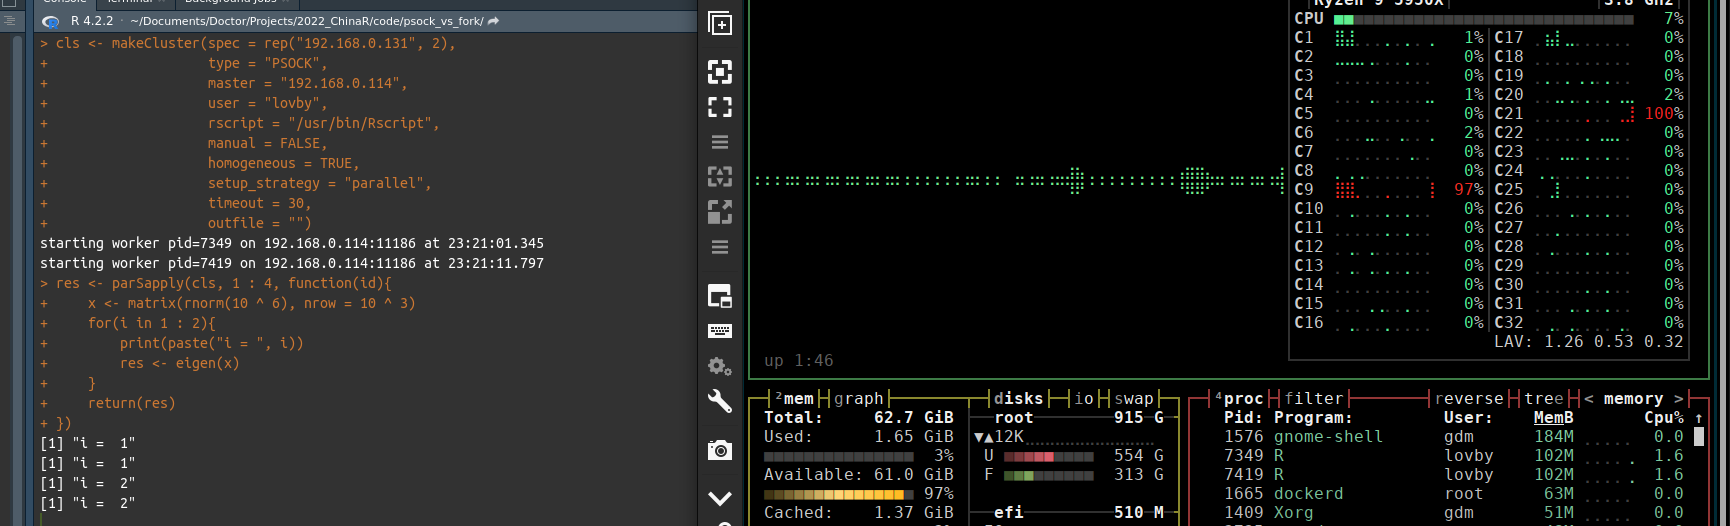
\includegraphics[width = \textwidth]{psock_remote}
    \caption{PSOCK connects to remote server}
  \end{figure}
\end{frame}

\begin{frame}
  \frametitle{Rabbit hole 1: PSOCK vs FORK}
  \begin{figure}[htbp]
    \centering
    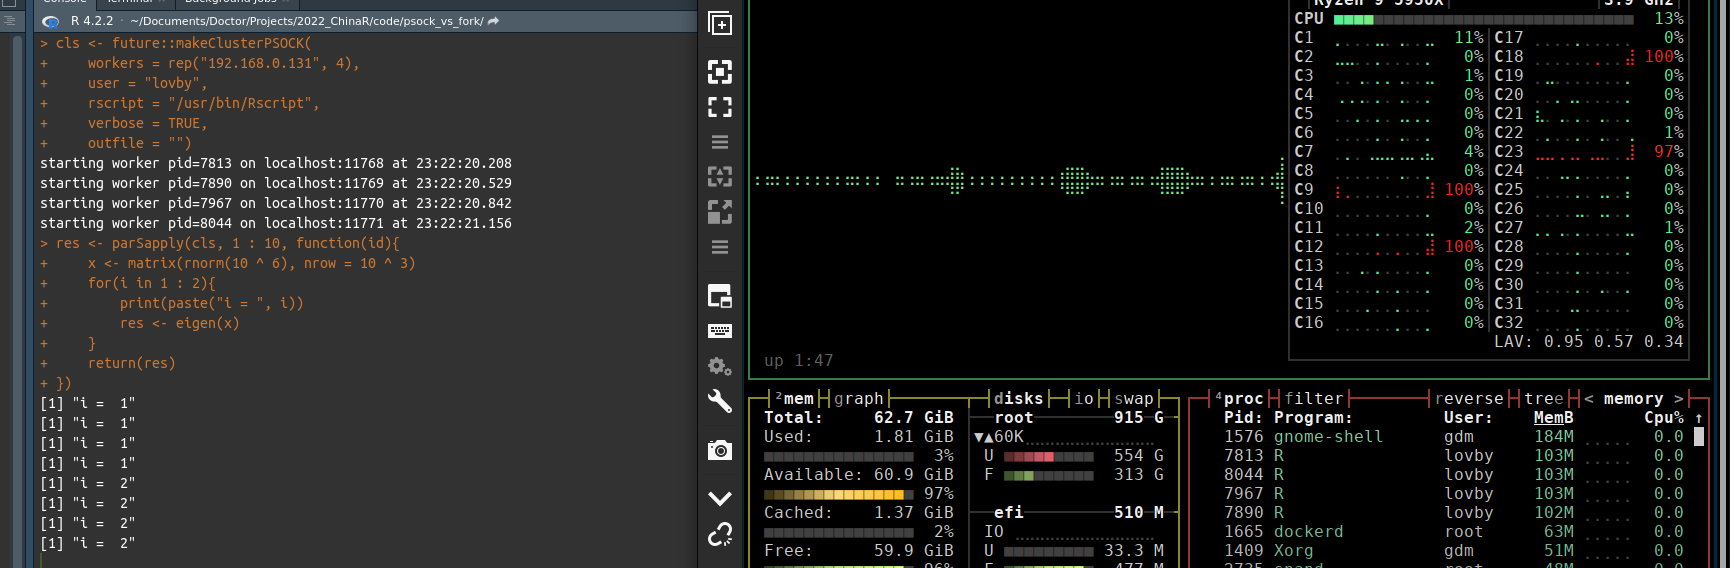
\includegraphics[width = \textwidth]{psock_remote_future}
    \caption{PSOCK (via future/parallely) connects to remote server}
  \end{figure}
\end{frame}

\begin{frame}
  \frametitle{Rabbit hole 1: PSOCK vs FORK}
  \begin{figure}[htbp]
    \centering
    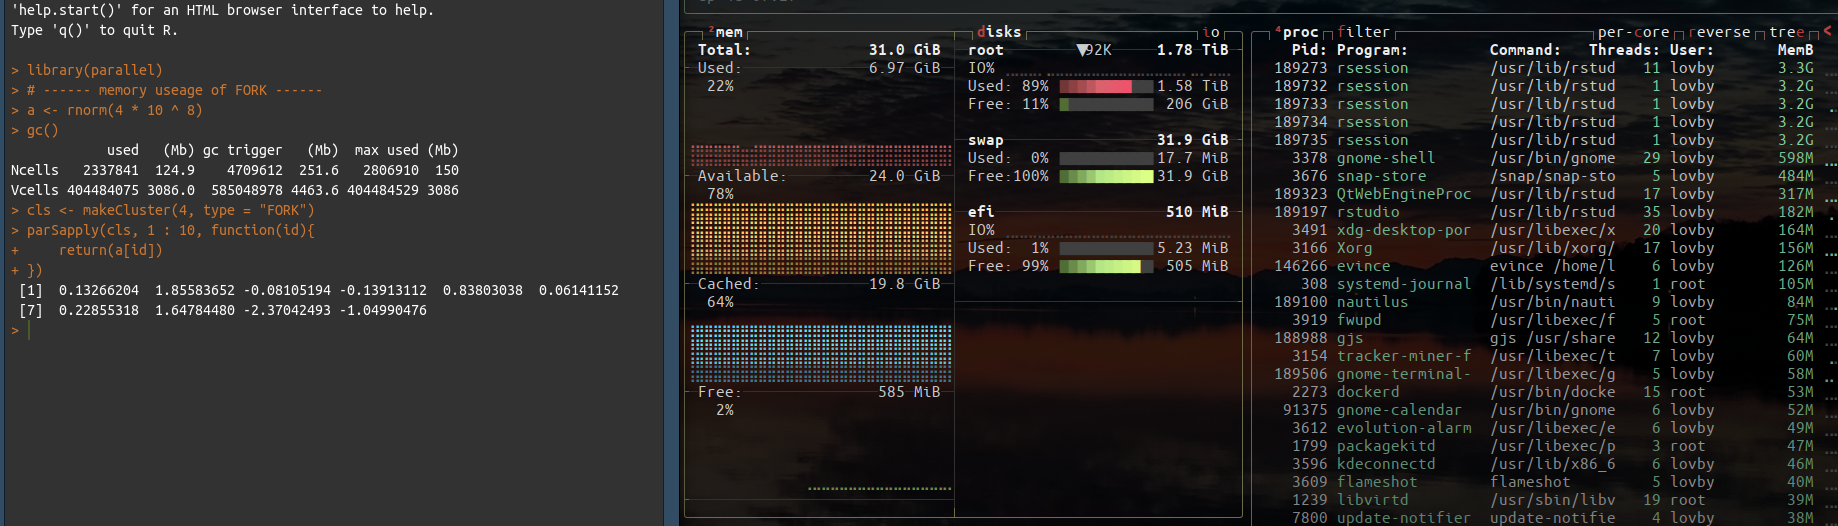
\includegraphics[width = \textwidth]{fork_start}
    \caption{Memory consumption of FORK, part 1}
  \end{figure}
\end{frame}

\begin{frame}
  \frametitle{Rabbit hole 1: PSOCK vs FORK}
  \begin{figure}[htbp]
    \centering
    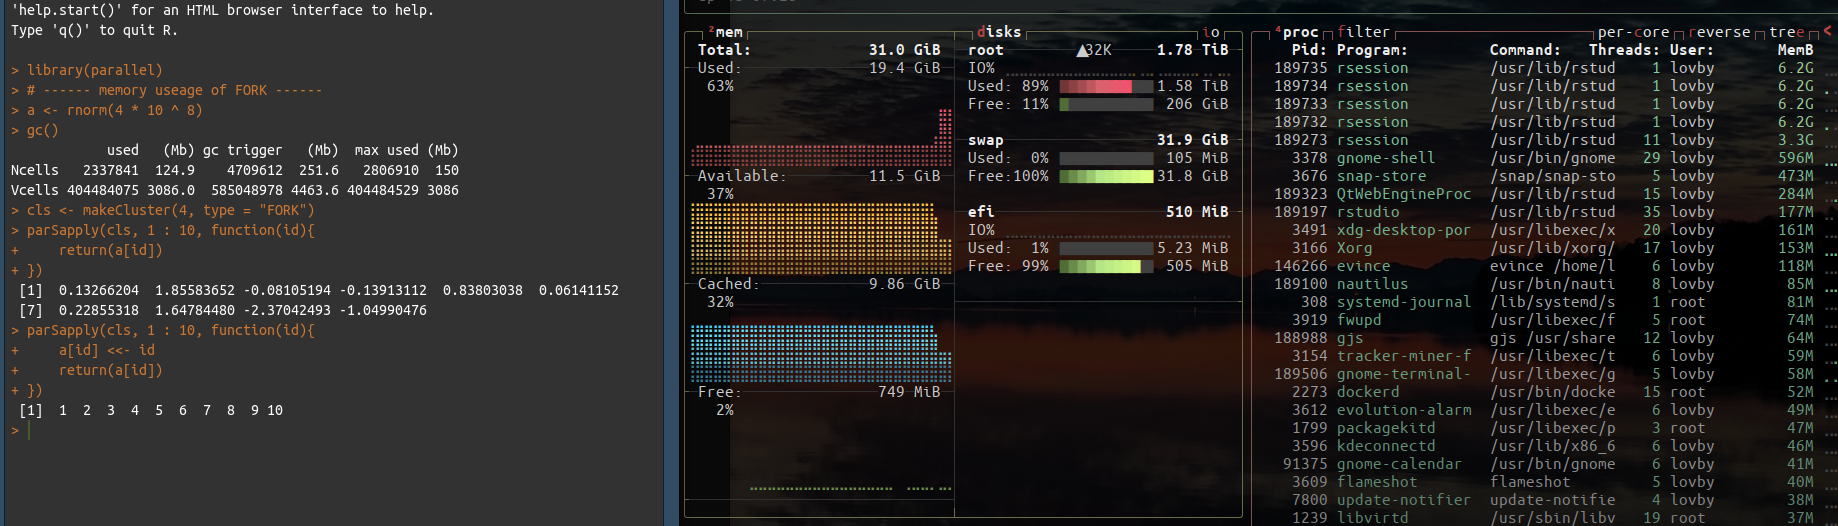
\includegraphics[width = \textwidth]{fork_transport}
    \caption{Memory consumption of FORK, part 2}
  \end{figure}
\end{frame}

\begin{frame}
  \frametitle{Rabbit hole 1: PSOCK vs FORK}
  \begin{block}{PSOCK}
    \begin{itemize}
    \item Pros:
      \begin{itemize}
      \item Use socket connection, a general approach.
      \item All system, locally or remotely with suitable setup such as MPI
      \end{itemize}
    \item Cons:
      \begin{itemize}
      \item Might be hard to configure.
      \item Manually transport the data.
      \end{itemize}
    \end{itemize}
  \end{block}
  \begin{block}{FORK}
    \begin{itemize}
    \item Pros: use FORK mechanism, no worry about variable transportation.
    \item Cons: Only for one machine, not available on Windows.
    \end{itemize}
  \end{block}
\end{frame}


\begin{frame}
  \frametitle{Rabbit hole 2: Parallel random number generation}
  \begin{figure}[htbp]
    \centering
    \begin{subfigure}[h]{0.45\textwidth}
      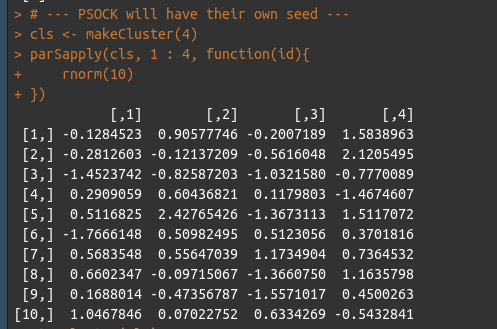
\includegraphics[width = \textwidth]{RNG_psock}
      \caption{No control on PSOCK}
    \end{subfigure}
        \begin{subfigure}[h]{0.45\textwidth}
      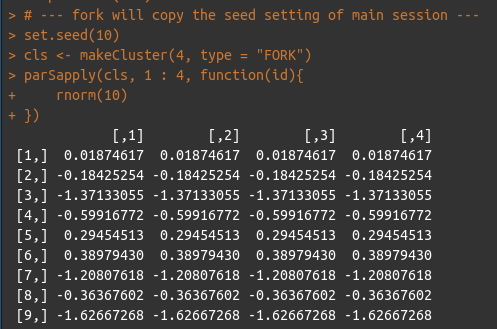
\includegraphics[width = \textwidth]{RNG_fork}
      \caption{Same seed on FORK}
    \end{subfigure}
  \end{figure}
\end{frame}

\begin{frame}
  \frametitle{Rabbit hole 2: Parallel random number generation}
  \begin{itemize}
  \item Manually use \mintinline{r}{set.seed()} on every worker. {\color{brown} not recommended}
  \item Use 'L’Ecuyer-CMRG' multiple RNG stream.
    \begin{enumerate}
    \item \mintinline{r}{RNGkind("L'Ecuyer-CMRG")} on your main session.
    \item \mintinline{r}{set.seed()} on your main session.
    \item \mintinline{r}{clusterSetupRNGstream()} to set your workers' seed.
    \end{enumerate}
  \end{itemize}
\end{frame}

\begin{frame}[fragile]
  \frametitle{Rabbit hole 3: Variable transportation}
  \begin{itemize}
  \item Explicit functions and variables will always be transported.
  \item FORK will copy the main session at creation.
  \item Others should be taken care of by hand.
  \item Additional configuration of \mintinline{r}{clusterExport} when nested in a function call.
  \end{itemize}
\end{frame}

\subsection{Easy parallel computation}
\begin{frame}
  \frametitle{How many frameworks can one developer maintains?}
  There are so many different parallel backends:
  \begin{itemize}
  \item snow
  \item multicore
  \item parallel
  \item MPI
  \item Redis
  \item Hadoop
  \item Spark
  \item Slurm
  \item ...
  \end{itemize}
  How to support them? How to maintain code?
\end{frame}

\begin{frame}[fragile]
  \frametitle{Foreach}
  \mintinline{r}{foreach} defines a simple but powerful framework for map/reduce parallel computation.
  \begin{block}{Package author/code writer}
    Decide {\color{Brown}which part of code} can run in parallel.
  \end{block}
  \begin{block}{End user}
    Decide {\color{Brown}how} to run in parallel based on their available resources.
  \end{block}
  \mintinline{r}{foreach} is syntactically structured in the form of a for loop. But actually it works like {\color{red}-apply} functions.
\end{frame}

\begin{frame}[fragile]
  \frametitle{Foreach}
\begin{minted}{r}
library(foreach)
# library(doParallel)
# registerDoParallel()
a <- 10
foreach(i = 1 : 12, j = 12 : 1, .combine = rbind) %dopar%{
    Sys.sleep(0.5)
    # print will be dropped when run in parallel
    print(paste("i = ", i, ", j = ", j, sep = ""))
    # 'a' is passed automatically
    data.frame(i, j, a)
}
\end{minted}
\end{frame}

\begin{frame}[fragile]
  \frametitle{future}
  \begin{itemize}
  \item \mintinline{r}{future} provides a simple and uniform way of evaluating R expressions asynchronously using various resources available to the user.
  \item Asynchronous computation. Not constrained by a for-loop or apply syntax.
    \end{itemize}
  \end{frame}


\begin{frame}[fragile]
  \frametitle{future}
\begin{minted}{r}
library(future)
plan(cluster)

x <- future({
    x <- matrix(rnorm(10 ^ 6), nrow = 10 ^ 3)
    for(i in 1 : 5){
        print(paste("i = ", i))
        res <- eigen(x) 
    }
    return(res)
}, seed = T)    # not block the main session

resolved(x)    # check whether the future is resolved
a <- rnorm(10)    # we can do other stuff at the main session
\end{minted}
\end{frame}

\begin{frame}[fragile]
  \frametitle{Futureverse}
  % https://www.futureverse.org/
  \par
  Available extensions for map-reduce:
    \begin{itemize}
    \item \mintinline{r}{future.apply}
    \item \mintinline{r}{doFuture}: backends for \mintinline{r}{foreach}, \mintinline{r}{BiocParallel} and \mintinline{r}{plyr}.
    \item \mintinline{r}{furrr}
    \end{itemize}
\end{frame}

\begin{frame}[fragile]
  \frametitle{Futureverse - future.apply}
\mintinline{r}{future.apply} provides worry-free parallel alternatives to base-R "apply" functions.
\begin{minted}{r}
library(future.apply)    # default plan is sequential
# plan(cluster)
x <- rnorm(16)
future_lapply(1 : 5, function(id){
    print(paste("id = ", id, sep = ""))    # normal print kept
    Sys.sleep(0.5)
    sum(x[1 : id])
})
\end{minted}
\end{frame}

\subsection{Other stuff}
\begin{frame}
  \frametitle{Personal suggestions}
  \begin{itemize}
  \item Nested parallel is {\color{Brown}NOT} recommended. At least it should be done with careful configuration.
  \item \mintinline{r}{future.apply} vs \mintinline{r}{foreach}
    \begin{itemize}
    \item Familiar with \mintinline{r}{foreach}: just use the \mintinline{r}{doFuture} backends.
    \item New to parallel: \mintinline{r}{future.apply} is a good start point for your code.
    \item \mintinline{r}{future} backend will relay the printed messages.
    \item Performance in parallel are close, {\color{Brown} so-called}.
    \item Performance for sequential are slower than for-loop.
    \end{itemize}
  \end{itemize}
\end{frame}

\begin{frame}
  \frametitle{I want progress bars}
  \begin{itemize}
  \item \mintinline{r}{RcppProgress} allows to display a progress bar in the R console for long running computations taking place in c++ code, supports OpenMP.
  \item \mintinline{r}{pbapply} is a lightweight package that adds progress bar to vectorized R functions ('*apply'). It supports several parallel backends.
  \item \mintinline{r}{progress} shows ASCII progress bars. 
  \item \mintinline{r}{progressr} provides a minimal API for reporting progress updates in R.
    \begin{itemize}
    \item Developer is responsible for providing progress updates.
    \item End user decides if, when, and how progress should be presented. 
    \end{itemize}
  \end{itemize}
\end{frame}

\begin{frame}[fragile]
  \frametitle{progressr}
\begin{minted}{r}
library(progressr)
slow_sum <- function(x) {
    p <- progressr::progressor(along = x)
    sum <- 0
    for (kk in seq_along(x)) {
        Sys.sleep(0.5)
        sum <- sum + x[kk]
        p(message = sprintf("Added %g", x[kk]))
    }
    sum
}
# handlers("default")    # default handler is "txtprogressbar"
with_progress(y <- slow_sum(1:10))
handlers("progress")
with_progress(y <- slow_sum(1:10))
\end{minted}
\end{frame}

\begin{frame}[fragile]
  \frametitle{Profile parallel code (WIP)}
  \begin{figure}[htbp]
    \centering
    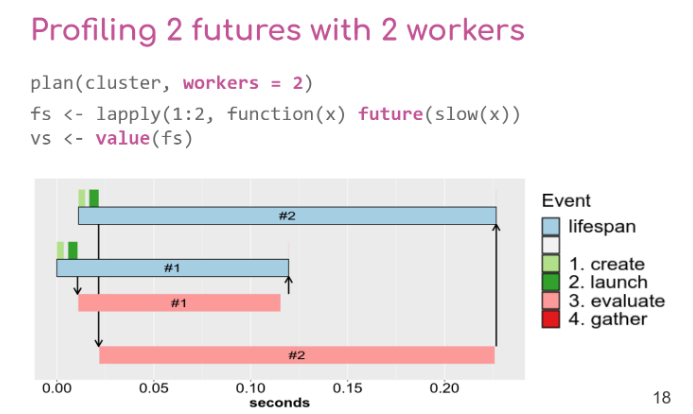
\includegraphics[width = 0.6\textwidth]{profile_future}
    \caption{Profile parallel code}
  \end{figure}
  Figure source at https://www.jottr.org/2022/06/23/future-user2022-slides/
\end{frame}

\begin{frame}[fragile]
  \frametitle{Profile parallel code (WIP)}
  \begin{minted}{r}
remotes::install_github(
    "git@github.com:HenrikBengtsson/future.git", 
    ref = "9875992", force = TRUE)
\end{minted}
  \begin{figure}[htbp]
    \centering
    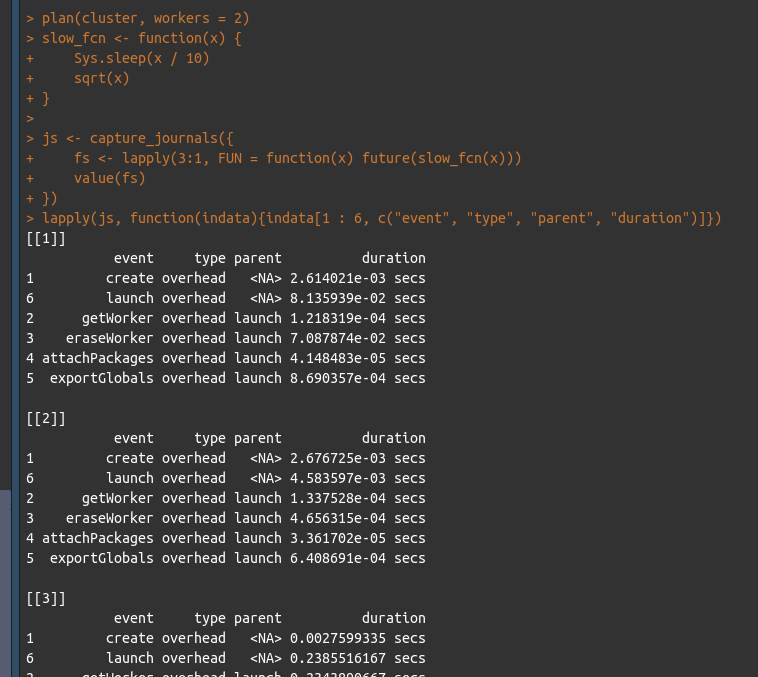
\includegraphics[width = 0.5\textwidth]{future_journal}
    \caption{Profile parallel code}
  \end{figure}
\end{frame}

\begin{frame}[fragile]
  \frametitle{Profile parallel code (WIP)}
\begin{minted}{r}
library(future)
n_worker <- 3
n <- 6

plan(cluster, workers = n_worker)
slow <- function(x){
    Sys.sleep(x / 5)
    return(x)
}

tmp <- capture_journals({
    fs <- lapply(1 : n, function(x) future(slow(x)))
    vs <- value(fs)  
})
\end{minted}
\end{frame}

\begin{frame}
  \frametitle{Profile parallel code (WIP)}
  \begin{figure}[htbp]
    \centering
    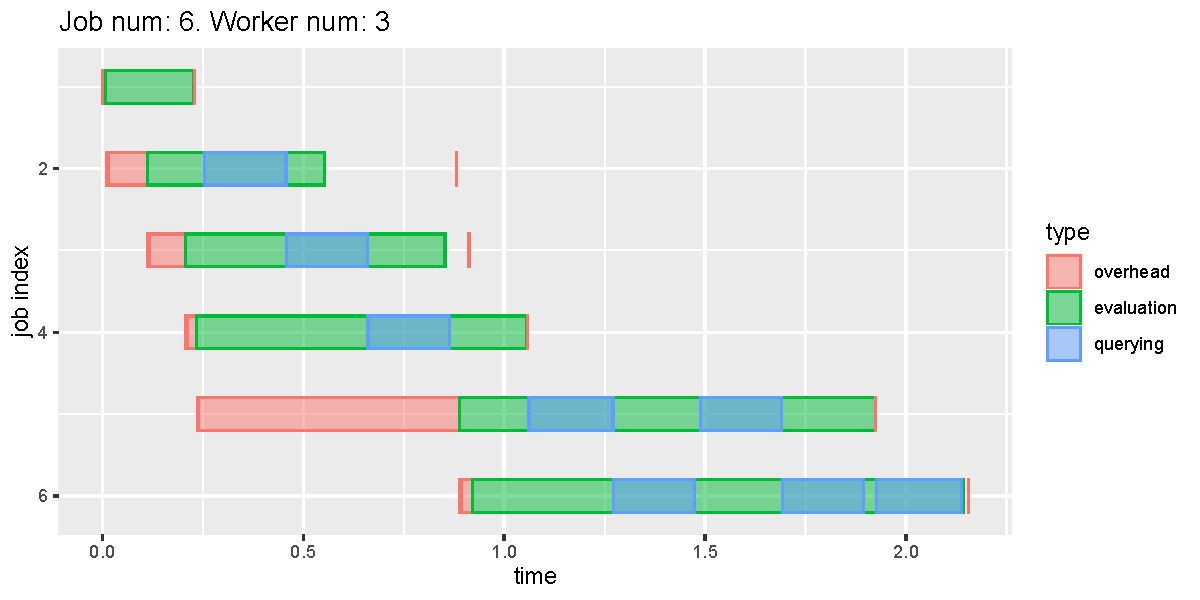
\includegraphics[width = 0.9\textwidth]{fig_type}
  \end{figure}
\end{frame}

\begin{frame}
  \frametitle{Profile parallel code (WIP)}
  \begin{figure}[htbp]
    \centering
    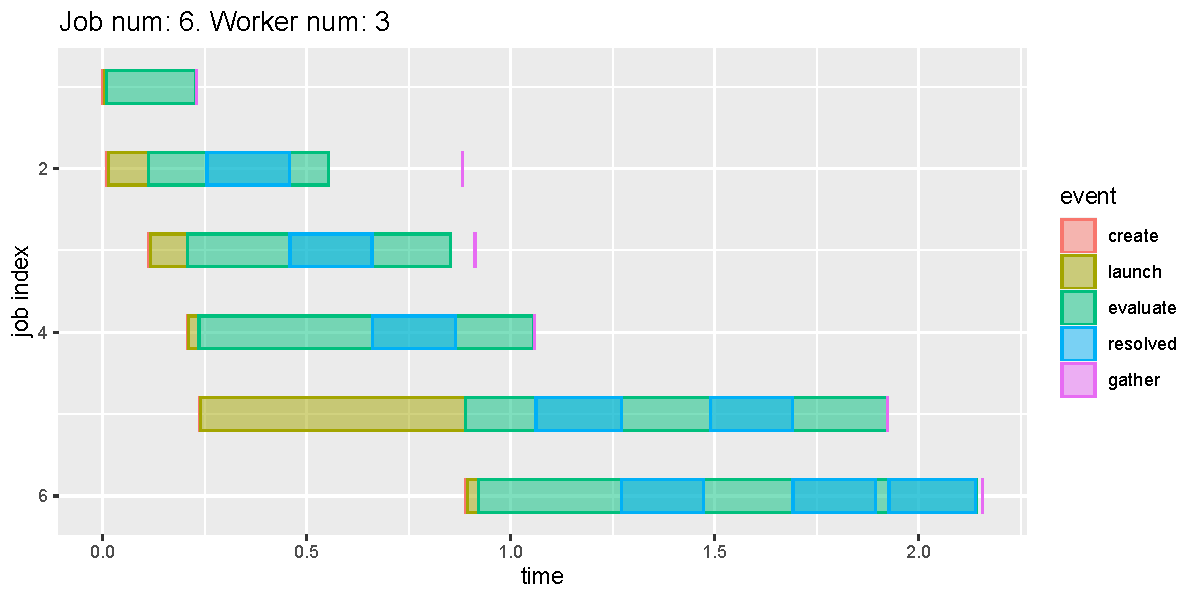
\includegraphics[width = 0.9\textwidth]{fig_event}
  \end{figure}
\end{frame}

\begin{frame}
  \frametitle{Profile parallel code (WIP)}
  \begin{figure}[htbp]
    \centering
    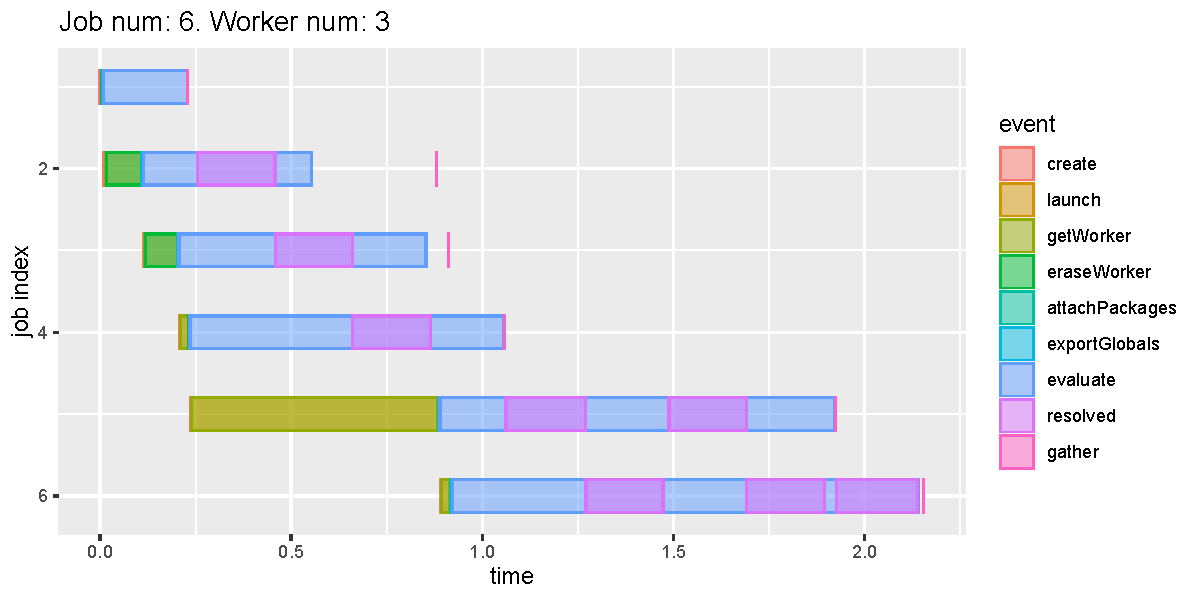
\includegraphics[width = 0.9\textwidth]{fig_event2}
  \end{figure}
\end{frame}

\begin{frame}
  \frametitle{Parallel is NOT all you need}
  How about we use $\frac{(1 + n) \times n}{2}$ ?
\end{frame}



% output message



\section{Acknowledgement}
{
  \setbeamercolor{background canvas}{bg=AliceBlue}
  \begin{frame}{Acknowledgement}
    \begin{figure}[htbp]
      \centering
      \begin{subfigure}[h]{0.4\textwidth}
        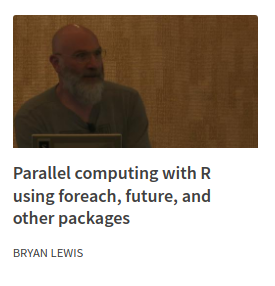
\includegraphics[width = \textwidth]{foreach_talk}
      \end{subfigure}
      \begin{subfigure}[h]{0.4\textwidth}
        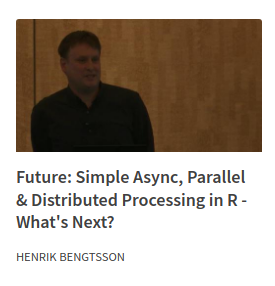
\includegraphics[width = \textwidth]{future_talk}
      \end{subfigure}
    \end{figure}
  \end{frame}
}
\end{document} 
%%% Local Variables:
%%% mode: latex
%%% TeX-master: t
%%% End:
